\section{Architektura Systemu}
\label{sec:Architektura_systemu}

Niniejszy rozdział opisuje zaprojektowaną architekturę systemu: jakie komponenty zostały wybrane, jak zostały ze sobą połączone i jakimi przesłankami kierowano się przy podejmowaniu kluczowych decyzji projektowych. Opis wdrożenia i szczegółów implementacji poszczególnych elementów zawarty jest w kolejnych rozdziałach.

\subsection{Cele i ograniczenia projektowe}

Projektując system, kierowano się czterema głównymi celami:

\begin{enumerate}
  \item \textbf{Pełna automatyzacja} --- dodanie nowych danych treningowych powinno wymagać wyłącznie wykonania polecenia \texttt{git push}; wszystkie dalsze kroki (walidacja, trening, ocena jakości, wdrożenie) powinny odbywać się bez udziału użytkownika.
  \item \textbf{Reprodukowalność} --- każda wersja modelu musi być jednoznacznie powiązana z wersją kodu, wersją danych treningowych i zapisanymi metrykami.
  \item \textbf{Kontrola kosztów} --- projekt realizowany jest w ramach akademickiego konta AWS z budżetem około 50~USD; zasoby obliczeniowe uruchamiane są tylko wtedy, gdy są faktycznie potrzebne.
  \item \textbf{Kontrola czasu} --- Labolatorium AWS może być uruchomione maksymalnie 4 godziny ciągiem, a trening modelu nie powinien przekraczać 2,5 godziny,aby umożliwić wykonanie pełnego cyklu CI/CD w ramach jednego uruchomienia.
  \item \textbf{Porównywalność} --- system musi umożliwiać zebranie mierzalnych danych (czas, koszt, liczba kroków manualnych) do porównania podejścia automatycznego z manualnym.
\end{enumerate}

Ograniczenia budżetowe miały bezpośredni wpływ na wybór technologii. Wykluczone zostały usługi zarządzane o wysokim koszcie stałym: Amazon EKS (zarządzany Kubernetes ~\$150/mies.), Amazon RDS (zarządzana baza danych), NAT Gateway (~\$32/mies.) oraz Application Load Balancer (~\$18/mies.). W ich miejsce zastosowano tańsze odpowiedniki: k3s na pojedynczej instancji EC2 zamiast EKS, SQLite jako backend MLflow zamiast RDS, oraz dostęp przez publiczny adres IP z NodePort zamiast load balancera. Szacowany koszt systemu przy typowym obciążeniu deweloperskim (kilka uruchomień tygodniowo) wynosi około 11~USD miesięcznie zakładając lekki ruch.

\subsection{Struktura repozytoriów}

Projekt korzysta z dwóch repozytoriów Git połączonych mechanizmem submodułów:

\begin{itemize}
  \item \textbf{Water-Meters-Segmentation-Autimatization} --- repozytorium główne, zawiera kod ML, metadane danych treningowych śledzone przez DVC, workflow GitHub Actions, konfigurację Docker i Helm oraz skrypty pomocnicze. Całość procesu CI/CD wyzwalana jest w tym repozytorium.
  \item \textbf{DevOps-AI-Model-Automatization} --- repozytorium infrastruktury, dołączone jako submoduł pod ścieżką \texttt{devops/}; zawiera moduły Terraform, skrypty konfiguracyjne EC2 oraz niniejszą pracę dyplomową.
\end{itemize}

Podział na dwa repozytoria wynika z różnego rytmu zmian: kod ML i dane zmieniają się często i wyzwalają automatyczne procesy, natomiast definicja infrastruktury zmienia się rzadko i jest zarządzana ręcznie. Dzięki mechanizmowi submodułów konkretna wersja infrastruktury jest powiązana z konkretną wersją kodu aplikacji, co zachowuje pełną reprodukowalność środowiska.

\begin{figure}[H]
\centering
\begin{tikzpicture}[
  repo/.style={
    draw, rounded corners=4pt,
    minimum width=8.2cm, text width=8cm,
    align=left, inner sep=8pt,
    font=\small\ttfamily
  },
  repolabel/.style={
    font=\footnotesize\sffamily\bfseries,
    fill=white, inner sep=2pt
  },
  arrow/.style={-{Stealth[length=7pt]}, thick},
  dasharrow/.style={-{Stealth[length=7pt]}, thick, dashed, gray}
]

% --- Repozytorium główne ---
\node[repo, fill=blue!6] (main) {
  \textbf{Water-Meters-Segmentation-Autimatization} \quad {\normalfont\small\sffamily\textit{(repozytorium główne)}}\\[4pt]
  \textbullet\ WMS/\ \ --- kod ML, skrypty treningowe\\
  \textbullet\ .github/workflows/\ \ --- pipeline CI/CD\\
  \textbullet\ docker/,\ helm/\ \ --- konteneryzacja\\
  \textbullet\ WMS/data/training/\ \ --- dane (DVC)\\[2pt]
  \textbullet\ \textbf{devops/}\ \ \textit{$\leftarrow$ submoduł Git}
};

% --- Repozytorium infrastruktury (submoduł) ---
\node[repo, fill=orange!8, below=1.6cm of main] (infra) {
  \textbf{DevOps-AI-Model-Automatization} \quad {\normalfont\small\sffamily\textit{(submoduł)}}\\[4pt]
  \textbullet\ terraform/\ \ --- infrastruktura AWS\\
  \textbullet\ helm/ml-model/\ \ --- chart Kubernetes\\
  \textbullet\ scripts/\ \ --- skrypty automatyzacji\\
  \textbullet\ Thesis/\ \ --- niniejsza praca dyplomowa
};

% --- Repozytorium referencyjne ---
\node[repo, fill=gray!8, below=1.6cm of infra] (ref) {
  \textbf{Water-Meters-Segmentation} \quad {\normalfont\small\sffamily\textit{(referencja, tylko do odczytu)}}\\[4pt]
  \textbullet\ Oryginalny model U-Net (punkt wyjścia)\\
  \textbullet\ Metryki bazowe: Dice 0{,}9275,\ IoU 0{,}8865
};

% --- Strzałki ---
\draw[arrow] (main.south) -- node[right, font=\footnotesize\sffamily, xshift=4pt]
  {\texttt{git submodule}} (infra.north);

\draw[dasharrow] ([xshift=-1cm]infra.south) -- node[right, font=\footnotesize\sffamily, xshift=4pt]
  {orginalne repozytorium z modelem} ([xshift=-1cm]ref.north);

\end{tikzpicture}
\caption{Struktura repozytoriów projektu: repozytorium główne zawiera infrastrukturę jako submoduł Git; repozytorium referencyjne dostarcza oryginalny model i metryki bazowe}
\label{fig:repo-structure}
\end{figure}


\subsection{Warstwy architektury}

System zorganizowany jest w cztery logiczne warstwy, które razem tworzą kompletny pipeline MLOps. Rysunek~\ref{fig:architecture-overview} przedstawia ich wzajemne powiązania.

\begin{figure}[H]
\centering
\IfFileExists{img/03_architektura_systemu/C4.pdf}{%
  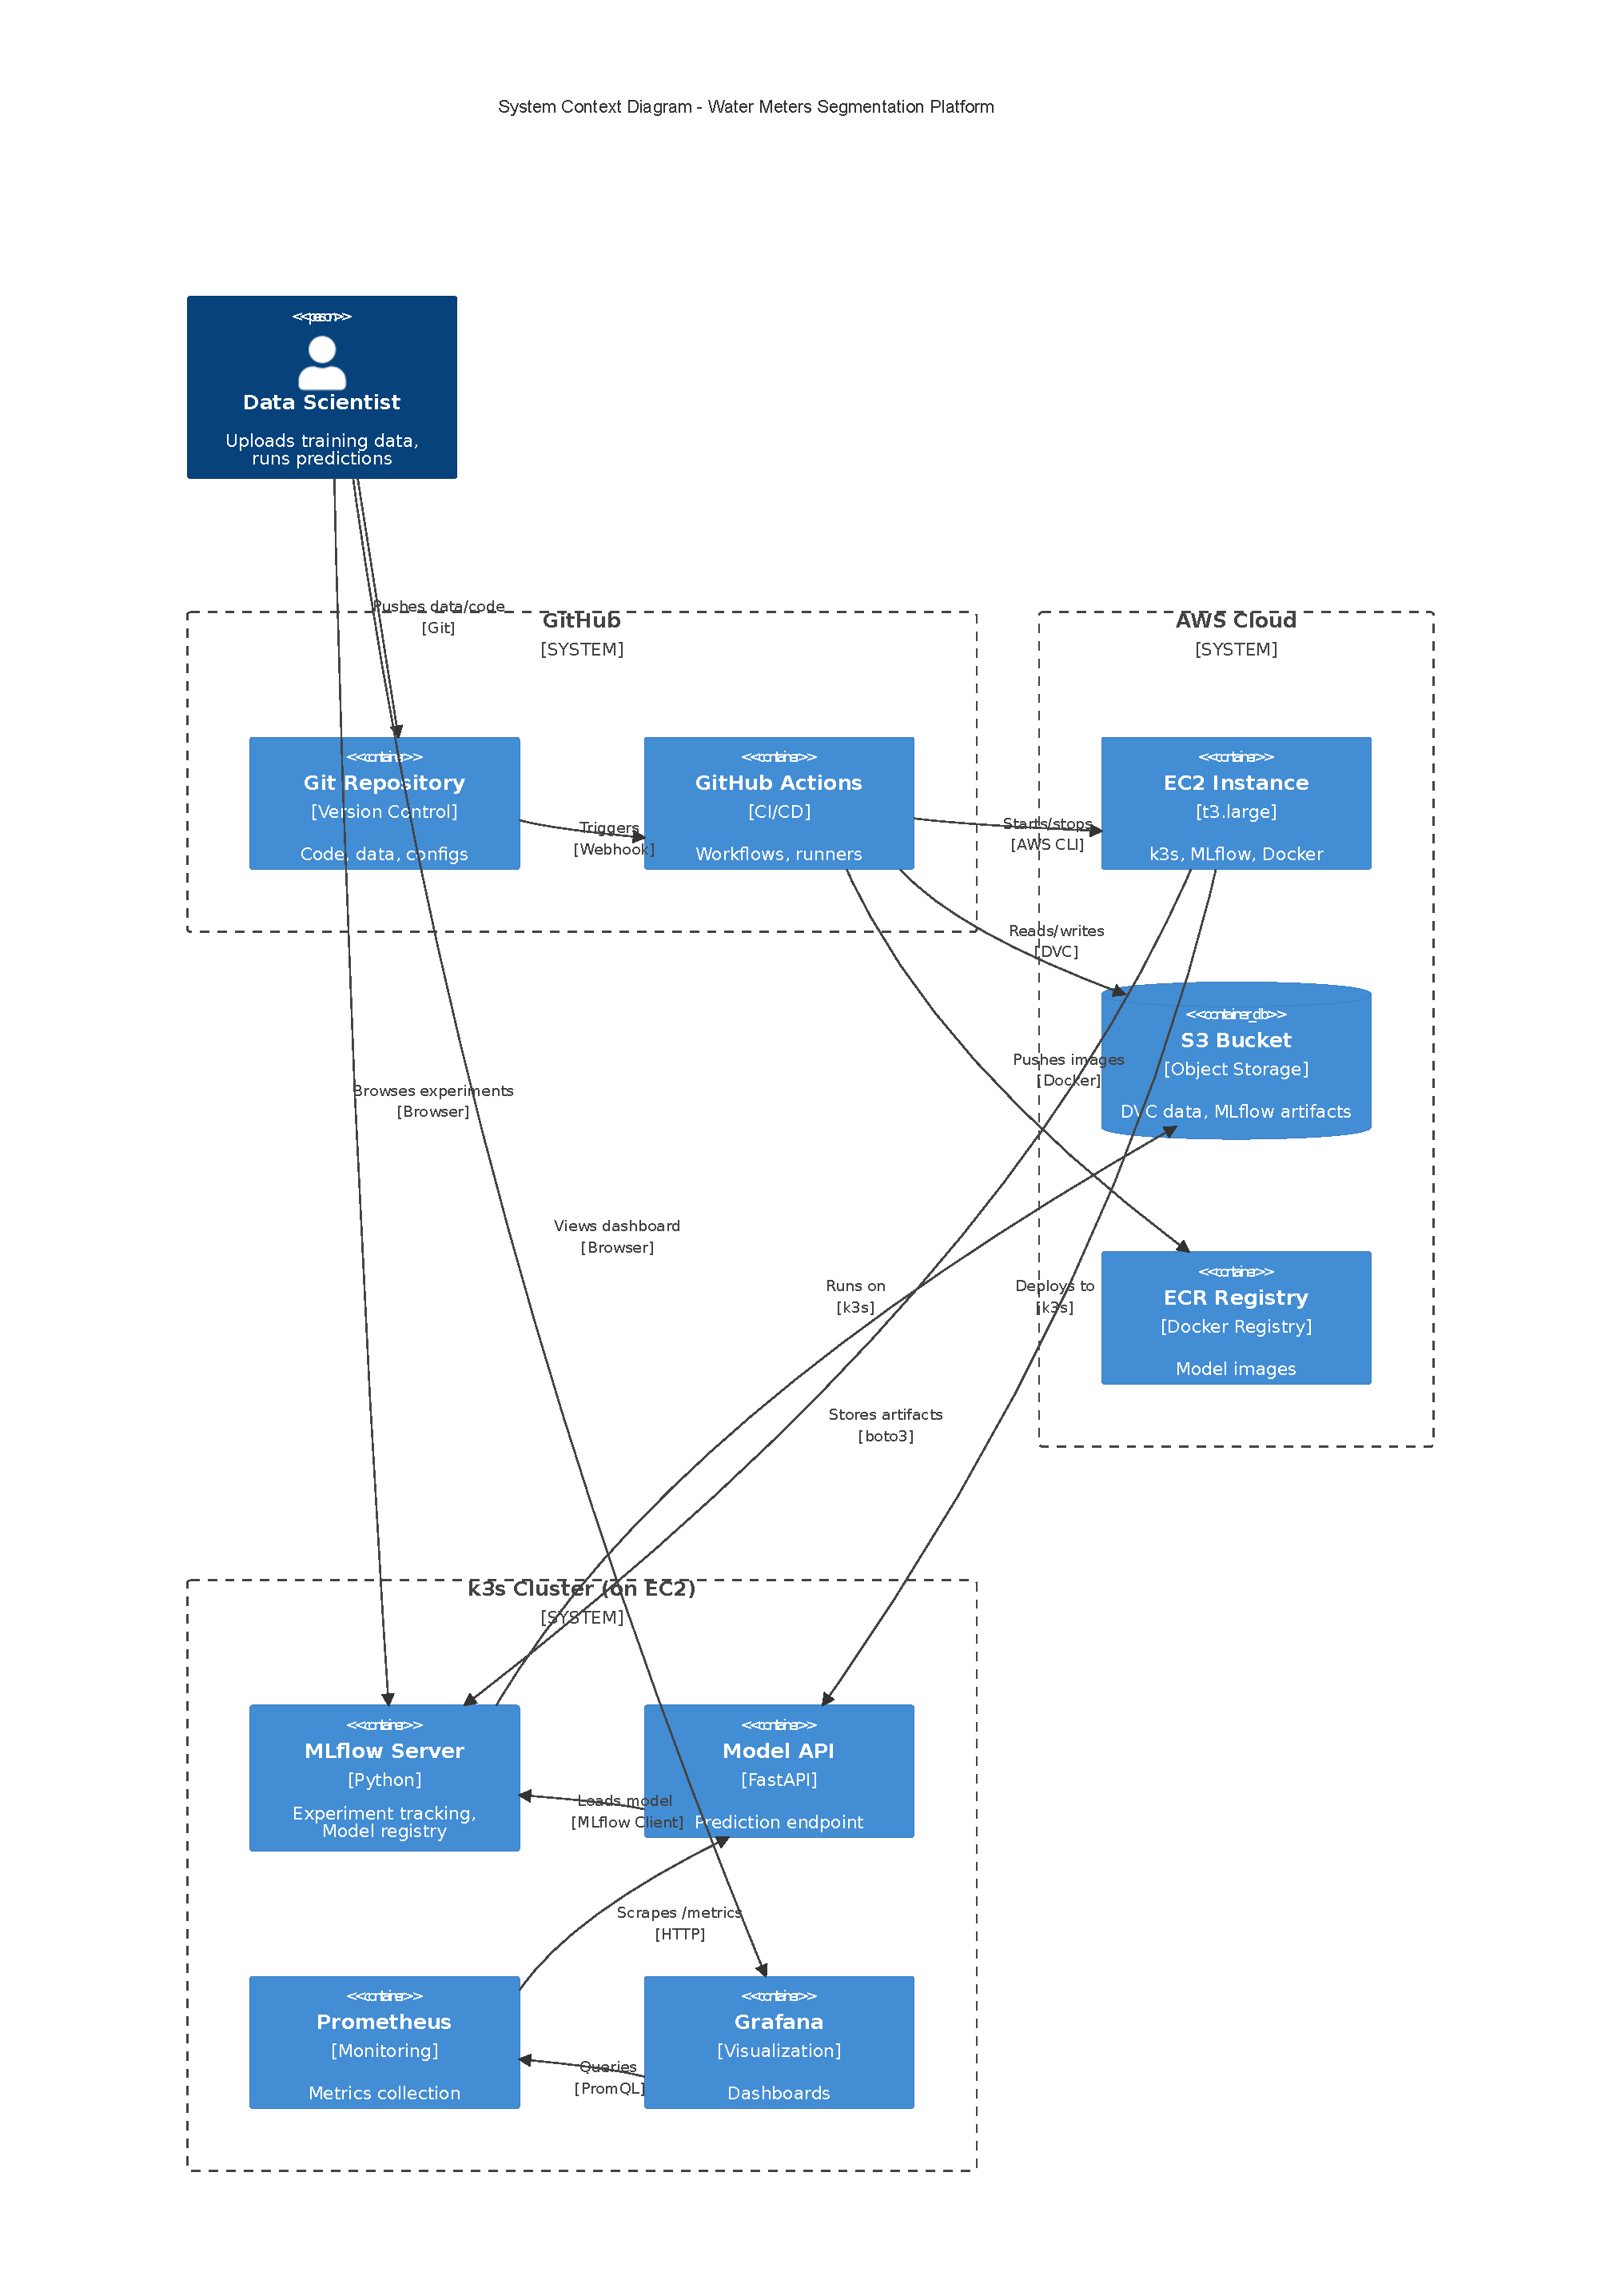
\includegraphics[width=\textwidth]{img/03_architektura_systemu/C4.pdf}%
}{%
  \fbox{\parbox{0.9\textwidth}{\centering\vspace{1.5cm}%
    \textit{[Diagram C4: główne komponenty systemu i ich interakcje]}%
  \vspace{1.5cm}}}%
}
\caption{Architektura systemu --- cztery warstwy i ich komponenty}
\label{fig:architecture-overview}
\end{figure}

% TODO: Diagram C4 wstawić jako C4.pdf (lub C4.png) do img/03_architektura_systemu/
% Diagram powinien pokazywać 4 warstwy (bloki poziome lub pionowe):
%   1. Kontrola wersji: Git/GitHub, DVC -> S3 (dane), Terraform/Helm (IaC)
%   2. Automatyzacja: GitHub Actions (workflow), hook pre-push
%   3. Infrastruktura AWS: EC2 (Elastic IP), S3 (DVC + MLflow), ECR
%   4. Aplikacja: k3s, MLflow Server, API modelu (FastAPI), Prometheus+Grafana
% Ze strzałkami między warstwami: git push -> Actions -> EC2 -> S3/ECR -> k3s

\subsubsection{Warstwa kontroli wersji}

Git i GitHub są centralnym punktem całego systemu --- każda zmiana, czy to w kodzie, danych czy infrastrukturze, przechodzi przez repozytorium. Repozytorium przechowuje kod ML, definicje pipeline'u i infrastruktury, natomiast same pliki binarne danych treningowych przechowywane są w S3 i śledzone przez DVC. Mechanizm \texttt{pre-push hook} automatycznie kieruje nowe dane treningowe na oddzielną gałąź, inicjując cały dalszy proces. Szczegóły działania hooka opisano w rozdziale~\ref{sec:Pipeline_CICD}.

\subsubsection{Warstwa automatyzacji}

GitHub Actions orkiestruje cały cykl życia modelu. Reaguje na pojawienie się nowej gałęzi danych i sekwencyjnie wywołuje: walidację danych, start infrastruktury, trening, bramkę jakości, wdrożenie (jeśli model poprawił się) oraz sprzątanie. Workflow korzysta z reużywalnych składników dla operacji na EC2, co eliminuje powielanie konfiguracji. Szczegółowy opis pipeline'u zawarty jest w rozdziale~\ref{sec:Pipeline_CICD}.

\subsubsection{Warstwa infrastruktury chmurowej}

Cała infrastruktura AWS zdefiniowana jest jako kod w Terraform i tworzona powtarzalnie jednym poleceniem. Kluczowe zasoby to: instancja EC2 ze statycznym Elastic IP (niezbędnym przy cyklicznym stop/start), dwa zasobniki S3 (dane DVC i artefakty MLflow) oraz rejestr obrazów ECR. Instancja EC2 pełni podwójną rolę --- runner treningu podczas pipeline'u i węzeł klastra k3s podczas serwowania modelu. Konfigurację infrastruktury opisuje rozdział~\ref{sec:Wdrozenie_systemu}.

\subsubsection{Warstwa aplikacji i monitoringu}

Na instancji EC2 działa klaster k3s z wdrożonym API modelu (FastAPI, zarządzany przez Helm), serwerem MLflow (systemd) oraz opcjonalnym stosem monitoringu Prometheus~+~Grafana. Model pobierany jest z rejestru MLflow przy starcie kontenera, co oddziela obraz Docker od konkretnej wersji modelu. Szczegóły konfiguracji wdrożenia opisuje rozdział~\ref{sec:Wdrozenie_systemu}.

\subsection{Kluczowe decyzje projektowe}

Tabela~\ref{tab:decisions} zestawia najważniejsze decyzje projektowe podjęte podczas budowy systemu, wraz z uzasadnieniem wyboru i odrzuconą alternatywą. Każda z nich wynika z jednego lub więcej celów wymienionych w sekcji~\ref{sec:Architektura_systemu}.

\begin{table}[H]
\centering
\caption{Kluczowe decyzje architektoniczne}
\label{tab:decisions}
\begin{tabular}{p{3.5cm}p{3.8cm}p{4.2cm}}
\toprule
\textbf{Decyzja} & \textbf{Wybór} & \textbf{Uzasadnienie} \\
\midrule
Orchestracja kontenerów
  & k3s na EC2
  & EKS jest ~15$\times$ droższy; k3s wystarcza dla jednego węzła \\
\addlinespace
Backend MLflow
  & SQLite
  & RDS ~\$30/mies.; SQLite jest wystarczający dla małego projektu; dane Meta przechowywane na EC2 \\
\addlinespace
Dostęp do API
  & NodePort 30080
  & Load Balancer ~\$18/mies.; publiczny adres IP EC2 z Elastic IP jest wystarczający \\
\addlinespace
Tytuł instancji EC2
  & t3.large (8~GB RAM)
  & t3.small/medium: crash OOM przy pobieraniu obrazu PyTorch 8,69~GB; t3.large jest minimum \\
\addlinespace
Stop/start EC2
  & Automatyczny po każdym pipeline
  & EC2 działa tylko ~3--4~h na uruchomienie; oszczędność ~80\% kosztów vs. ciągłe działanie \\
\addlinespace
Dane treningowe w Git
  & Tylko metadane DVC
  & Duże pliki binarne spowalniają Git i przekraczają limity; S3 jest tańszy i skalowalny \\
\addlinespace
Trening przed PR
  & Trening $\rightarrow$ PR (jeśli lepszy)
  & PR tworzony przez bota nie wyzwala innych workflow (ograniczenie GitHub); kolejność eliminuje problem \\
\addlinespace
Baseline bramki jakości
  & Dynamiczny z MLflow
  & Hardkodowany baseline staje się nieaktualny po każdym treningu; MLflow zawsze zna aktualny Production \\
\addlinespace
IAM dla GitHub Actions
  & Tymczasowe klucze sesji
  & AWS Academy zabrania tworzenia ról IAM; OIDC niedostępne; klucze rotowane ręcznie \\
\bottomrule
\end{tabular}
\end{table}
